\documentclass[../../main.tex]{subfiles}

\begin{document}

    %% ======================== ENTFERNT AUF EMPFEHLUNG DES TUTORS ========================

    % Aufgrund der erhöhten technischen Umsetzungsgeschwindigkeit einer Eingabeleistungsänderung am Diodenlaser versuchen wir zunächst mittels Rasterung über eine konstante Temperatur $T$ Minima in der Funktion $P_{\textit{an}}\mapsto \textit{Tr}(P_{\textit{an}})(T)$ zu finden. Unsere Messergebnisse für $T\in\{22\si{\celsius}, 24\si{\celsius}, 26\si{\celsius}, 28\si{\celsius}, 30\si{\celsius}\}=:\mcT$ sind in Abbildung \ref{fig:1-2:Rasterung22deg} bis \ref{fig:1-2:Rasterung30deg} zu sehen. 
    %% \begin{figure}
    %%     \centering
    %%     \begin{subfigure}[t]{0.45\textwidth}
    %%         \centering
    %%         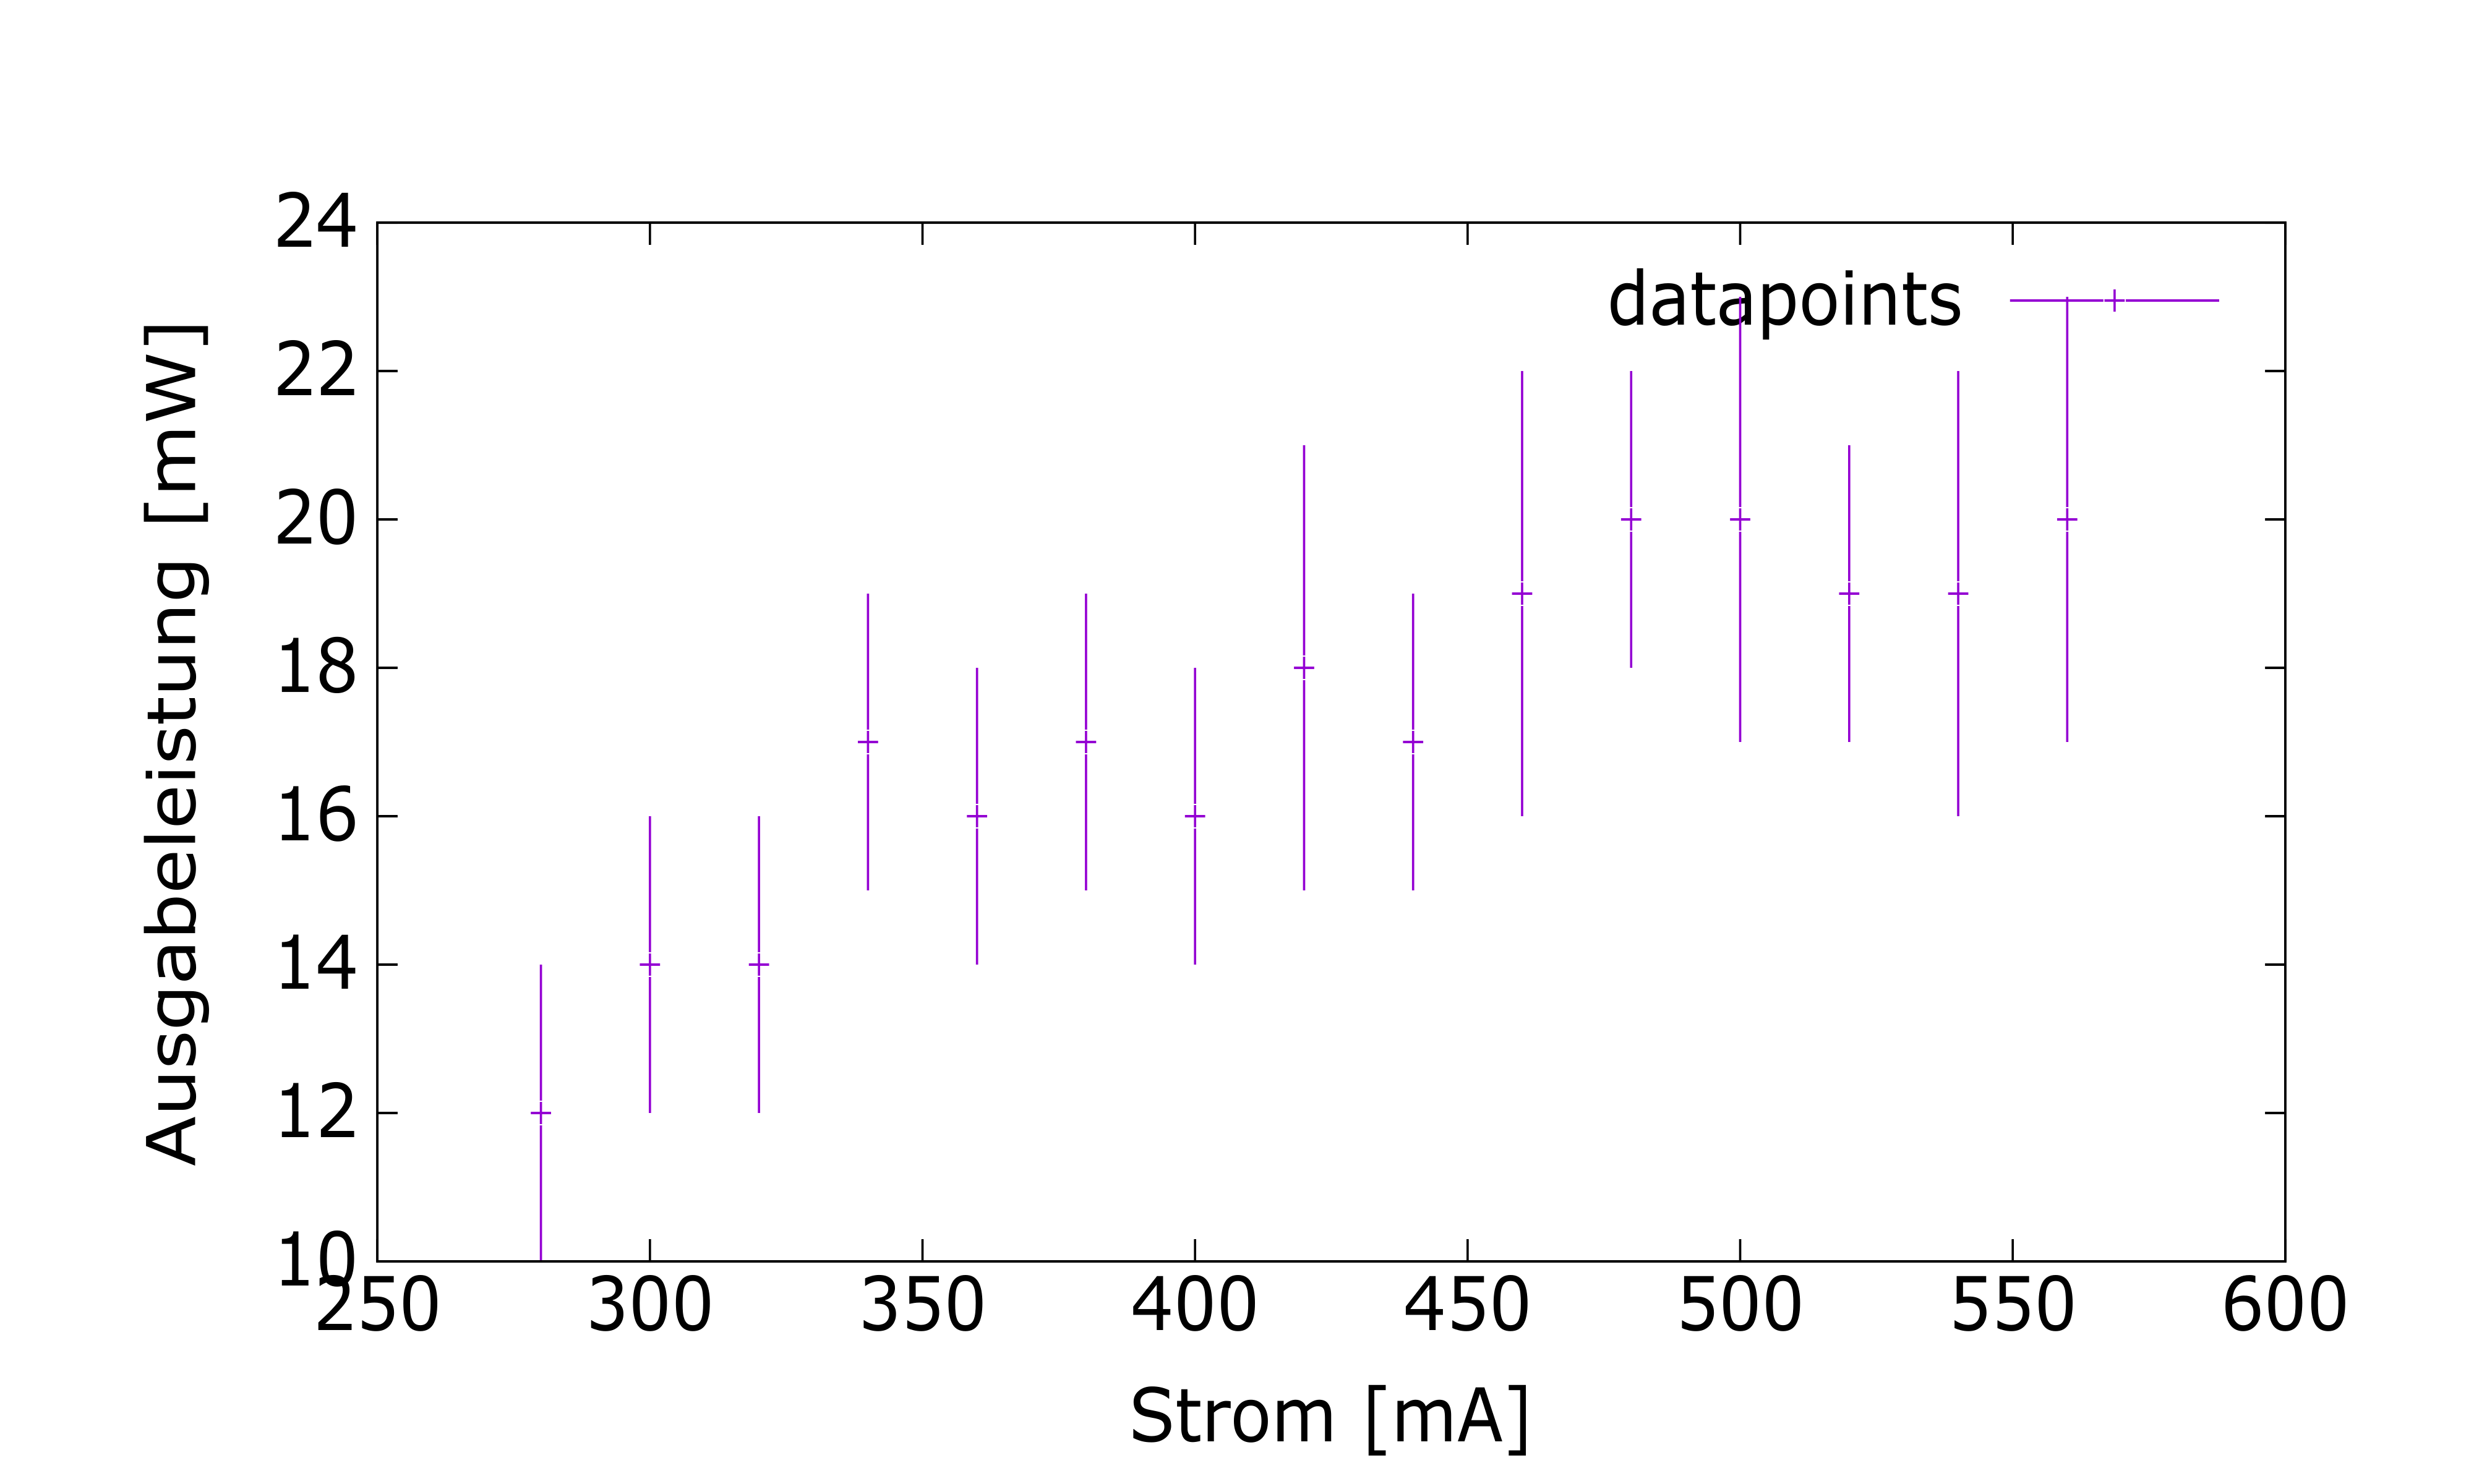
\includegraphics[width=\textwidth]{../../Bilddateien/1-2/Rasterung_22deg.png}
    %%         \caption{Rasterung um $22\si{\celsius}$.}
    %%         \label{fig:1-2:Rasterung22deg}
    %%     \end{subfigure}
    %%     \
    %%     \begin{subfigure}[t]{0.45\textwidth}
    %%         \centering
    %%         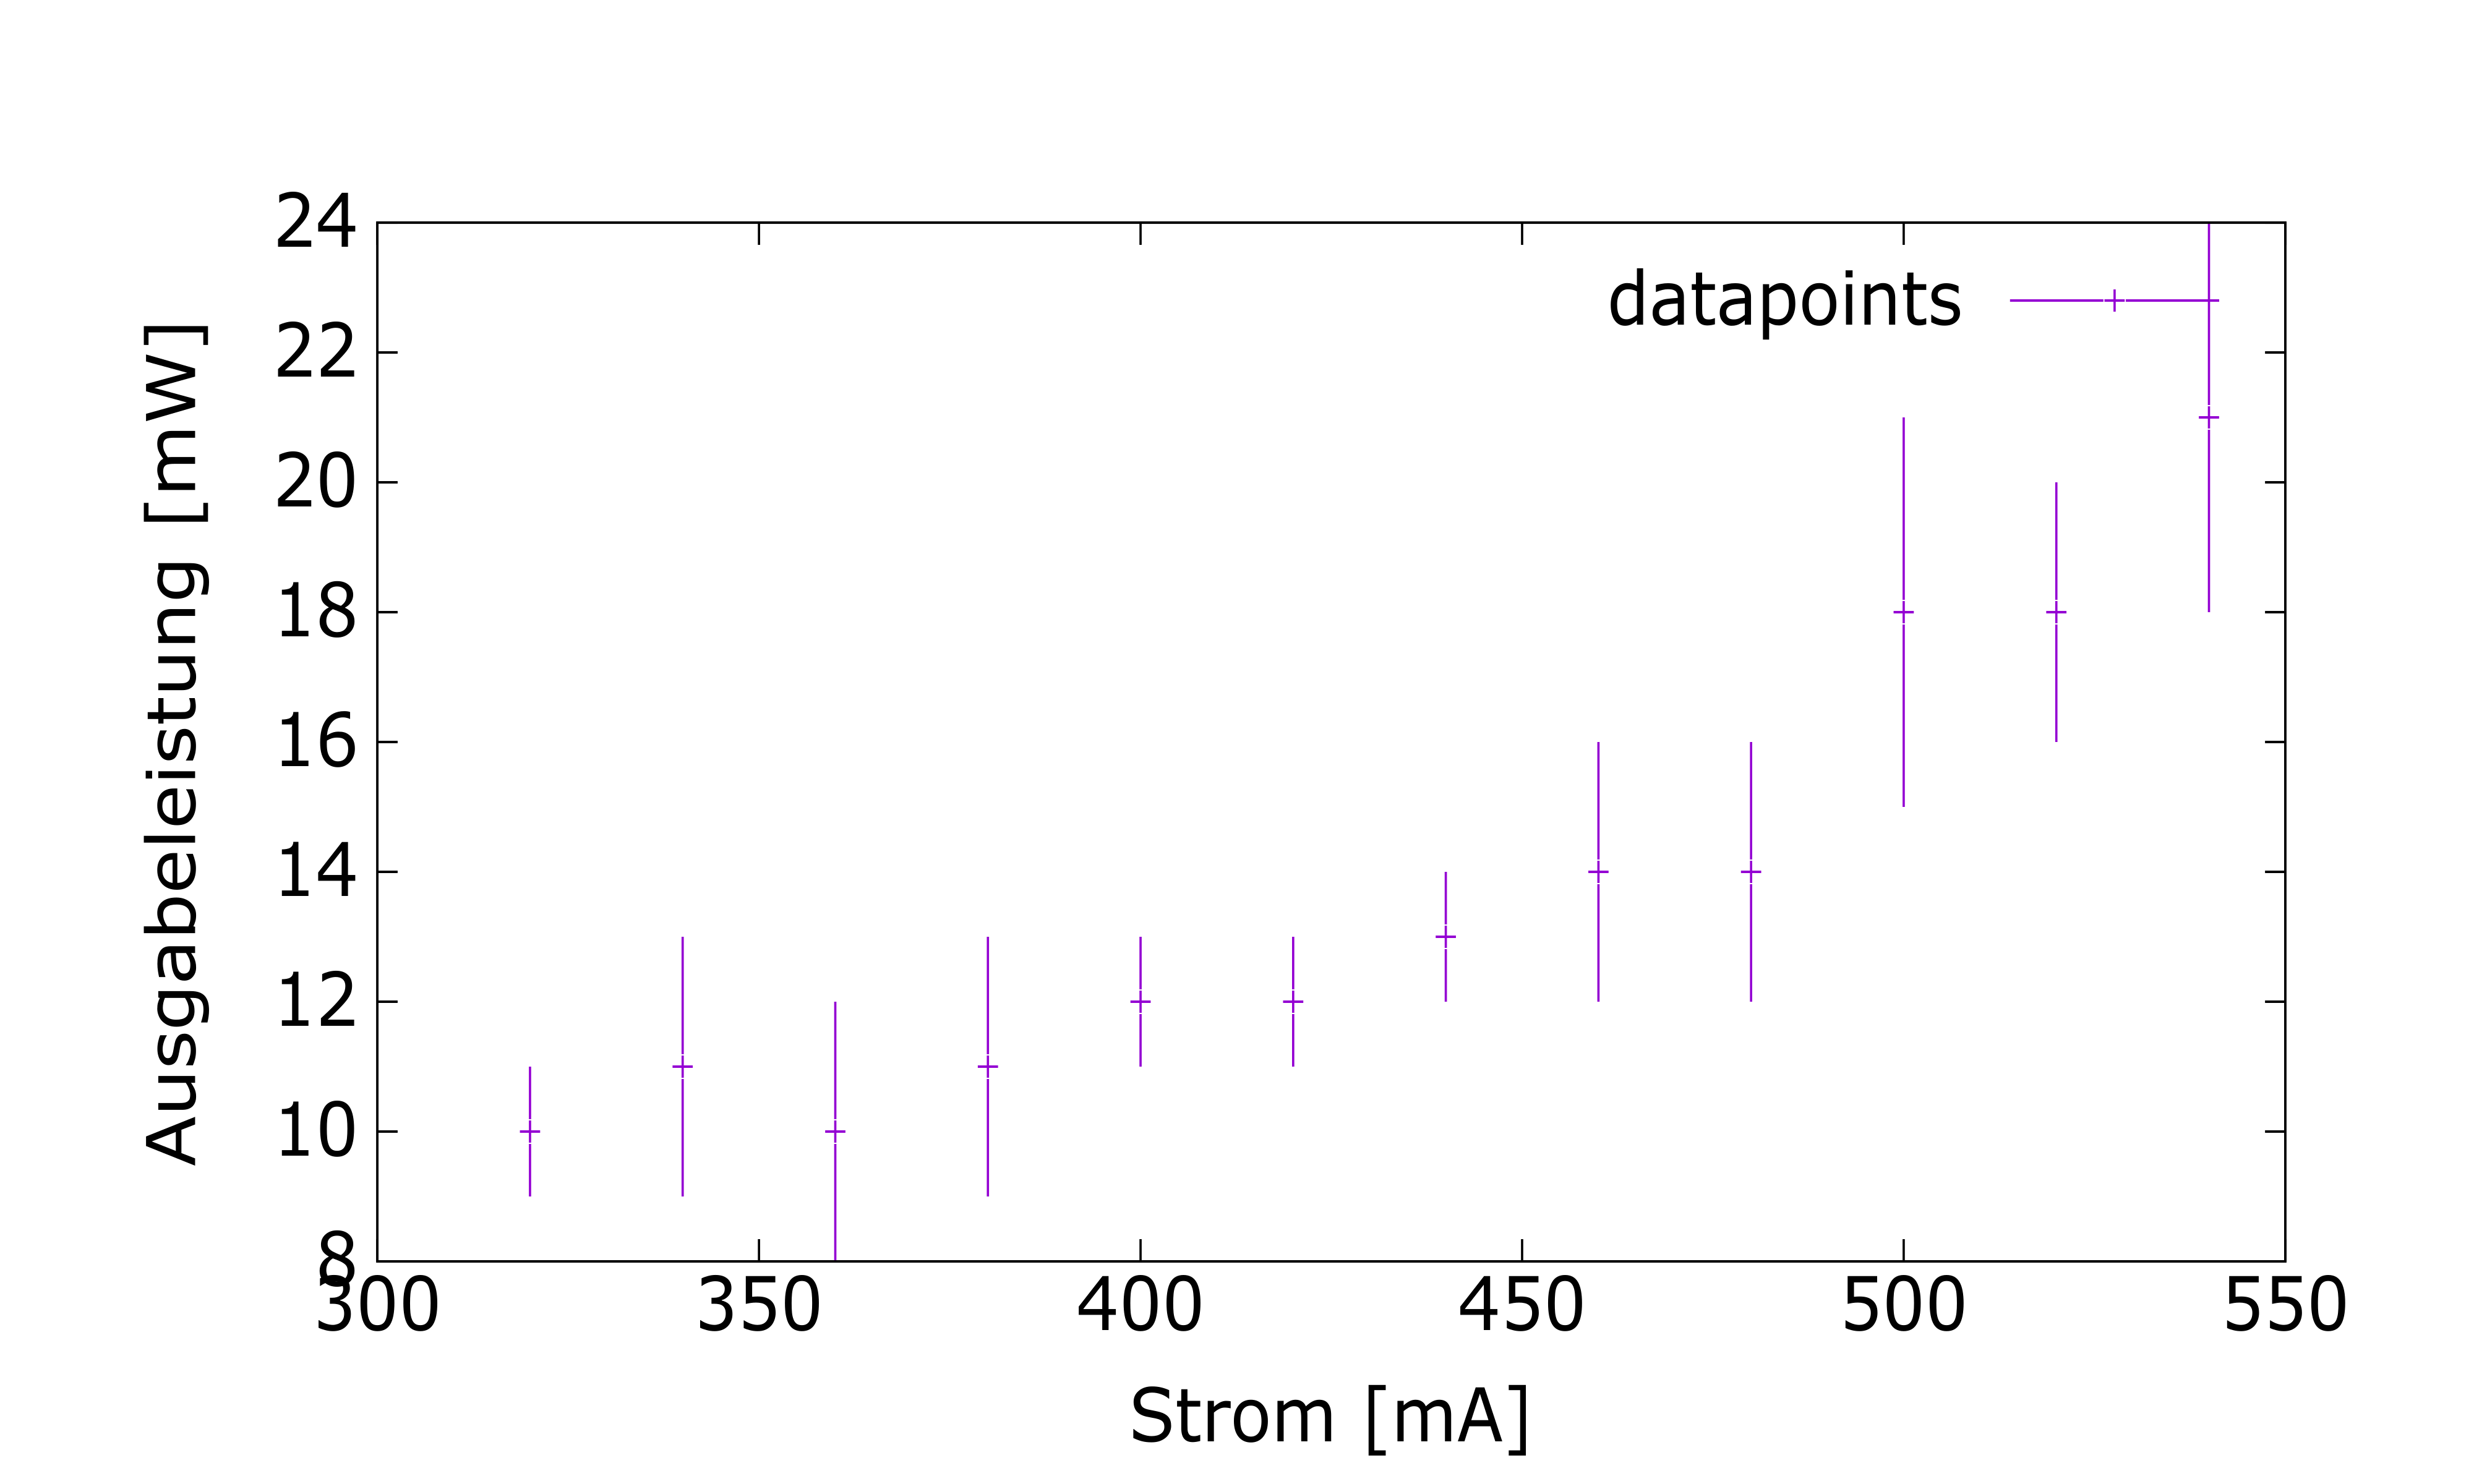
\includegraphics[width=\textwidth]{../../Bilddateien/1-2/Rasterung_24deg.png}
    %%         \caption{Rasterung um $24\si{\celsius}$.}
    %%         \label{fig:1-2:Rasterung24deg}
    %%     \end{subfigure}
    %%     \
    %%     \begin{subfigure}[t]{0.45\textwidth}
    %%         \centering
    %%         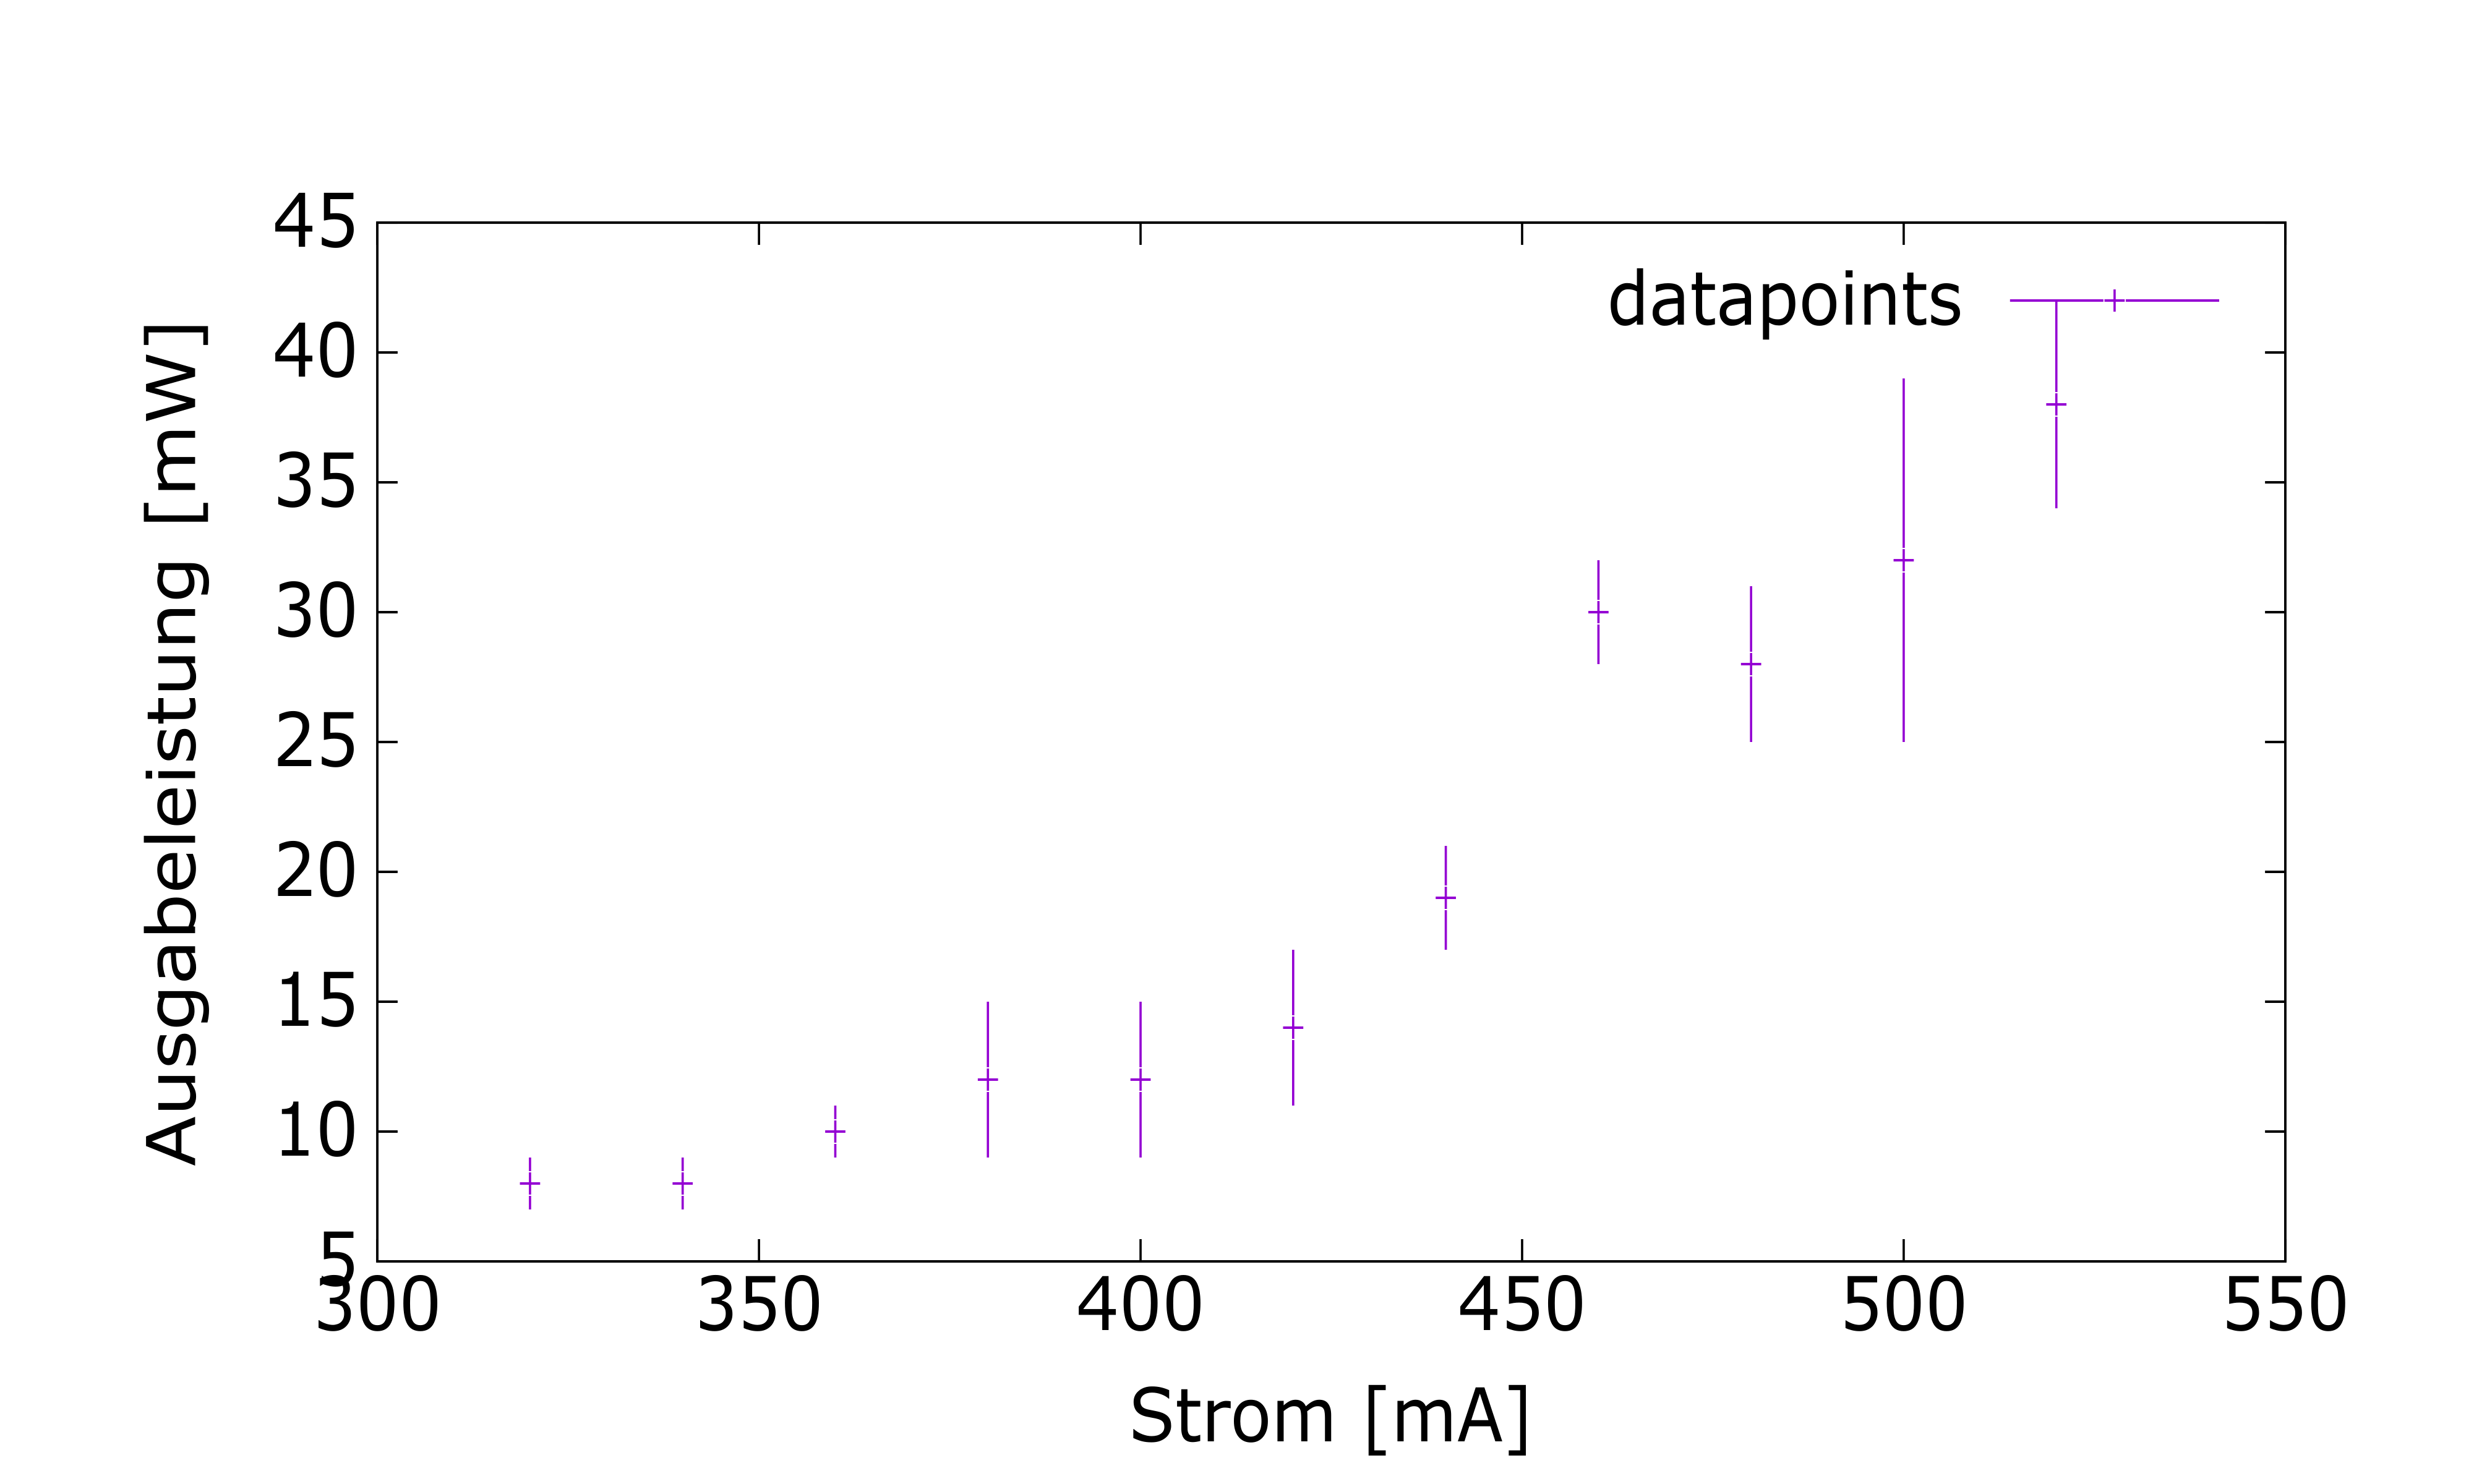
\includegraphics[width=\textwidth]{../../Bilddateien/1-2/Rasterung_26deg.png}
    %%         \caption{Rasterung um $26\si{\celsius}$.}
    %%         \label{fig:1-2:Rasterung26deg}
    %%     \end{subfigure}
    %%     \
    %%     \begin{subfigure}[t]{0.45\textwidth}
    %%         \centering
    %%         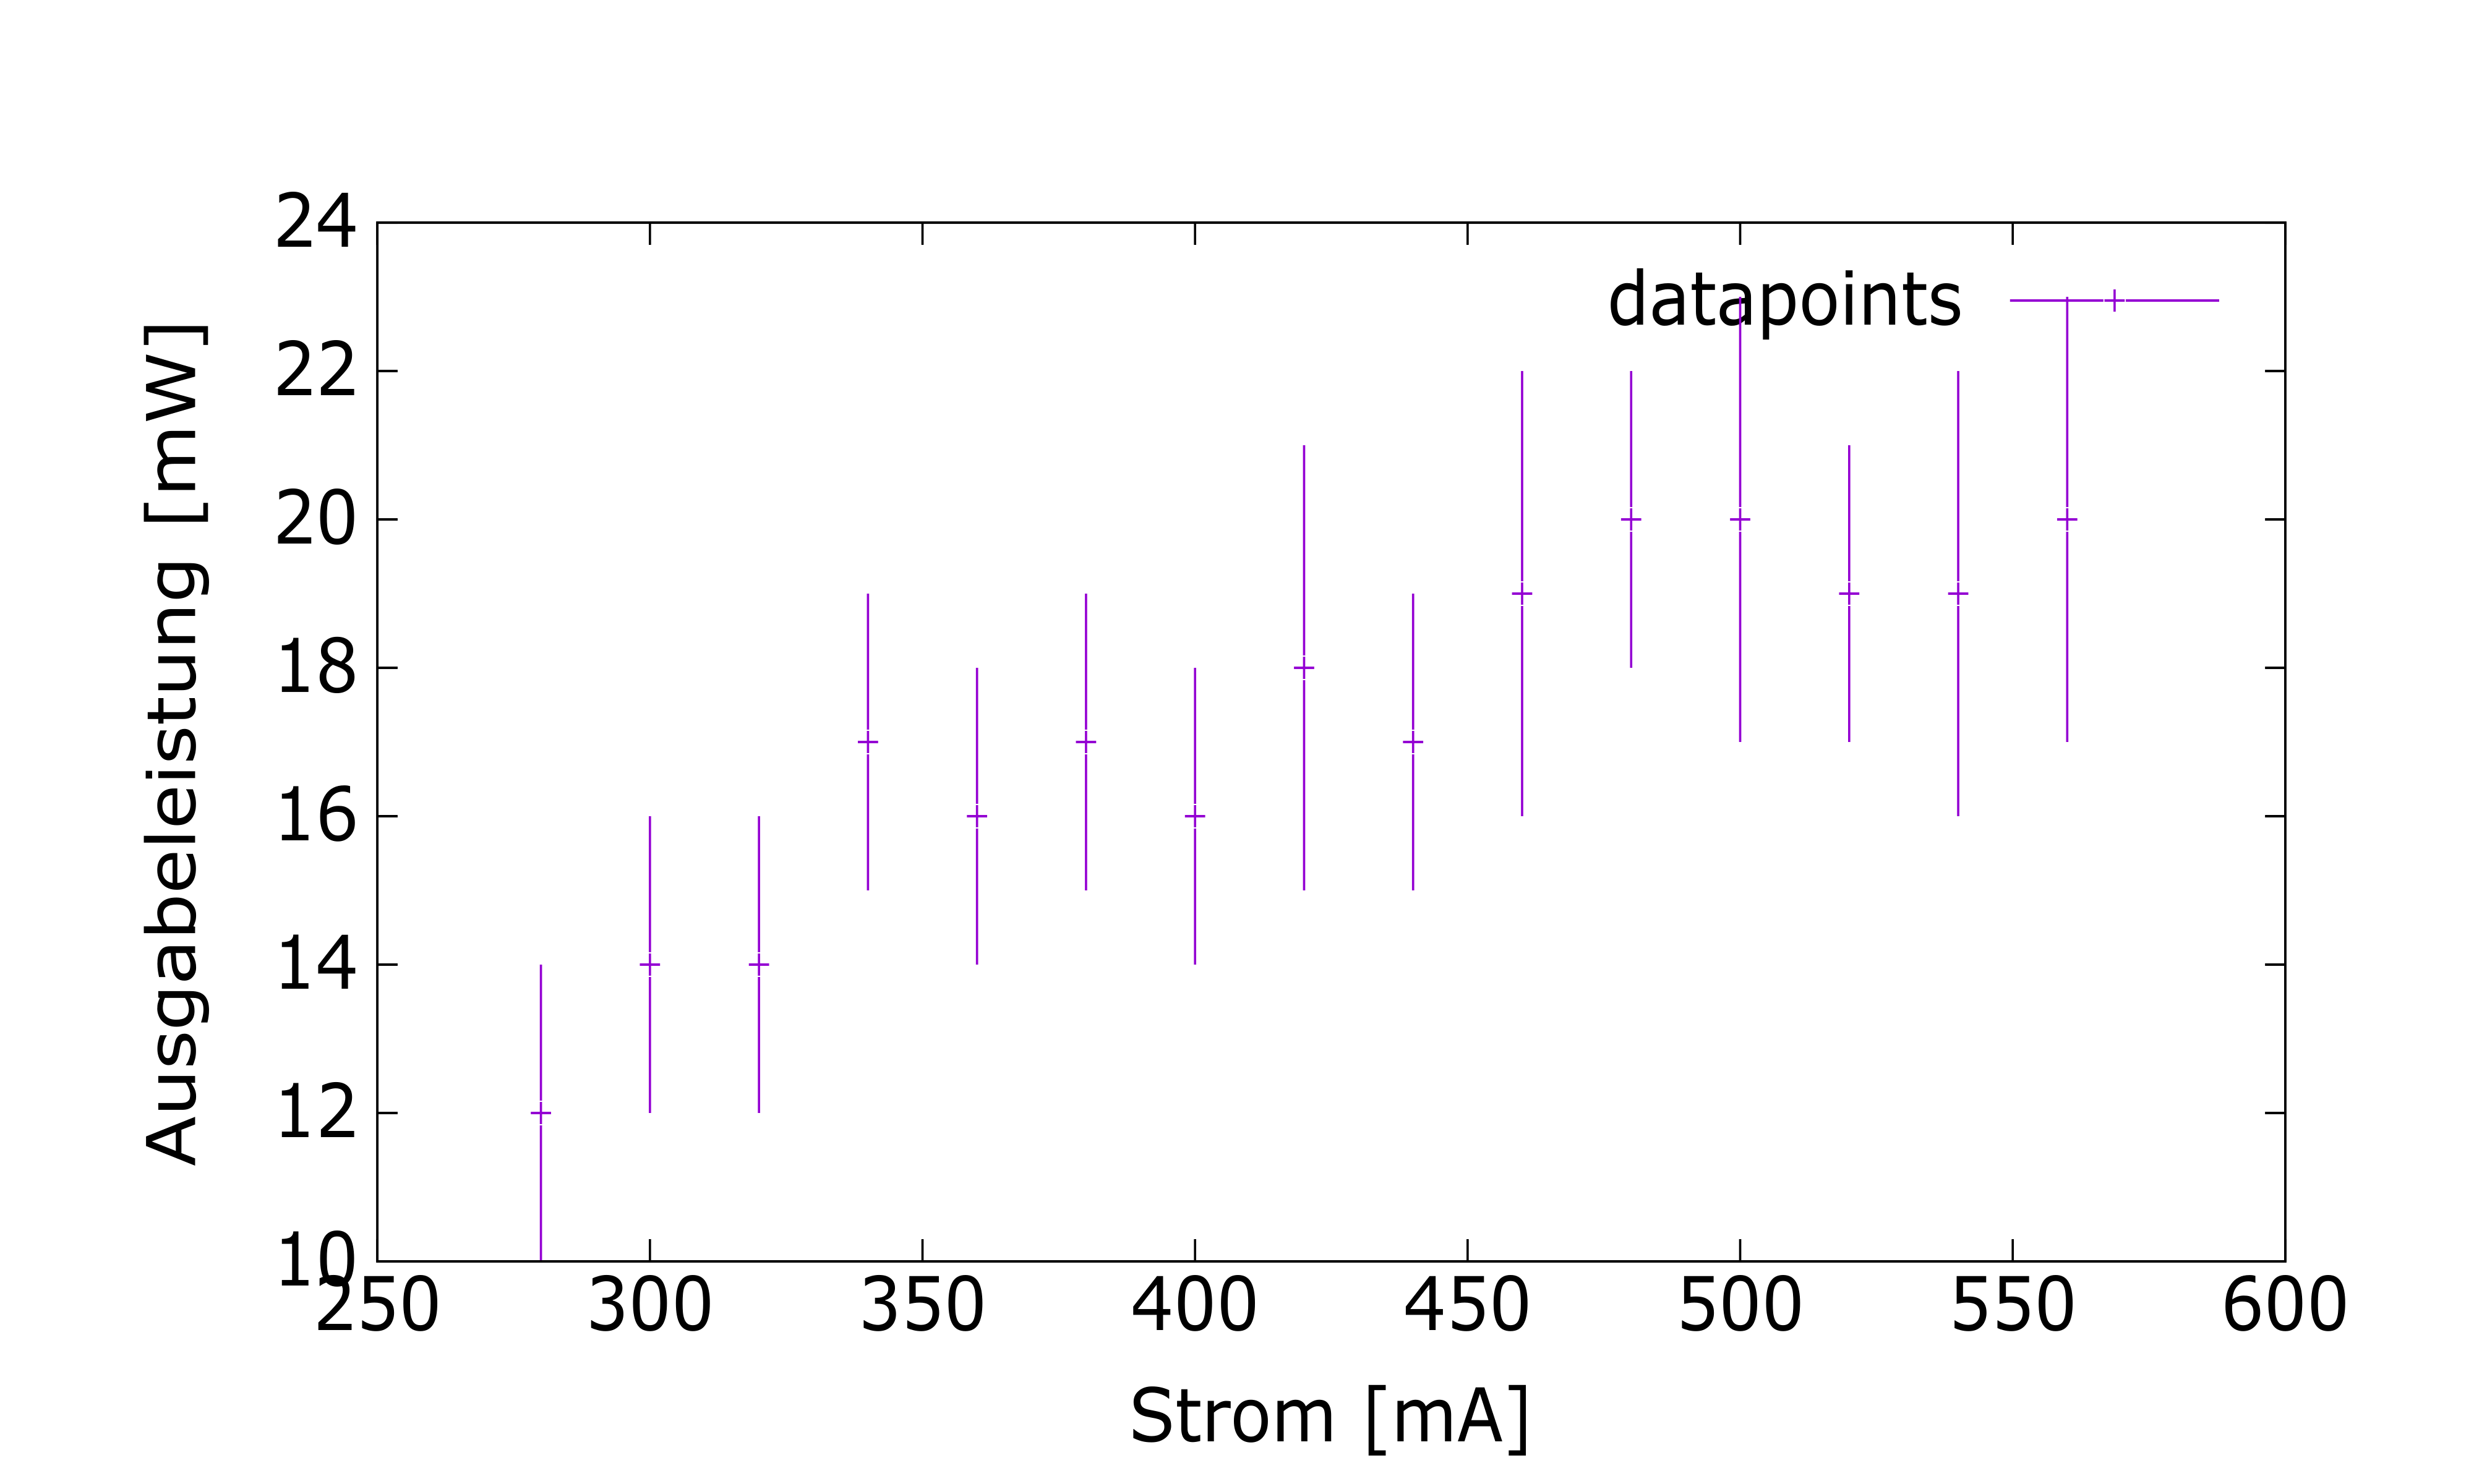
\includegraphics[width=\textwidth]{../../Bilddateien/1-2/Rasterung_28deg.png}
    %%         \caption{Rasterung um $28\si{\celsius}$.}
    %%         \label{fig:1-2:Rasterung28deg}
    %%     \end{subfigure}
    %%     \
    %%     \begin{subfigure}[t]{0.45\textwidth}
    %%         \centering
    %%         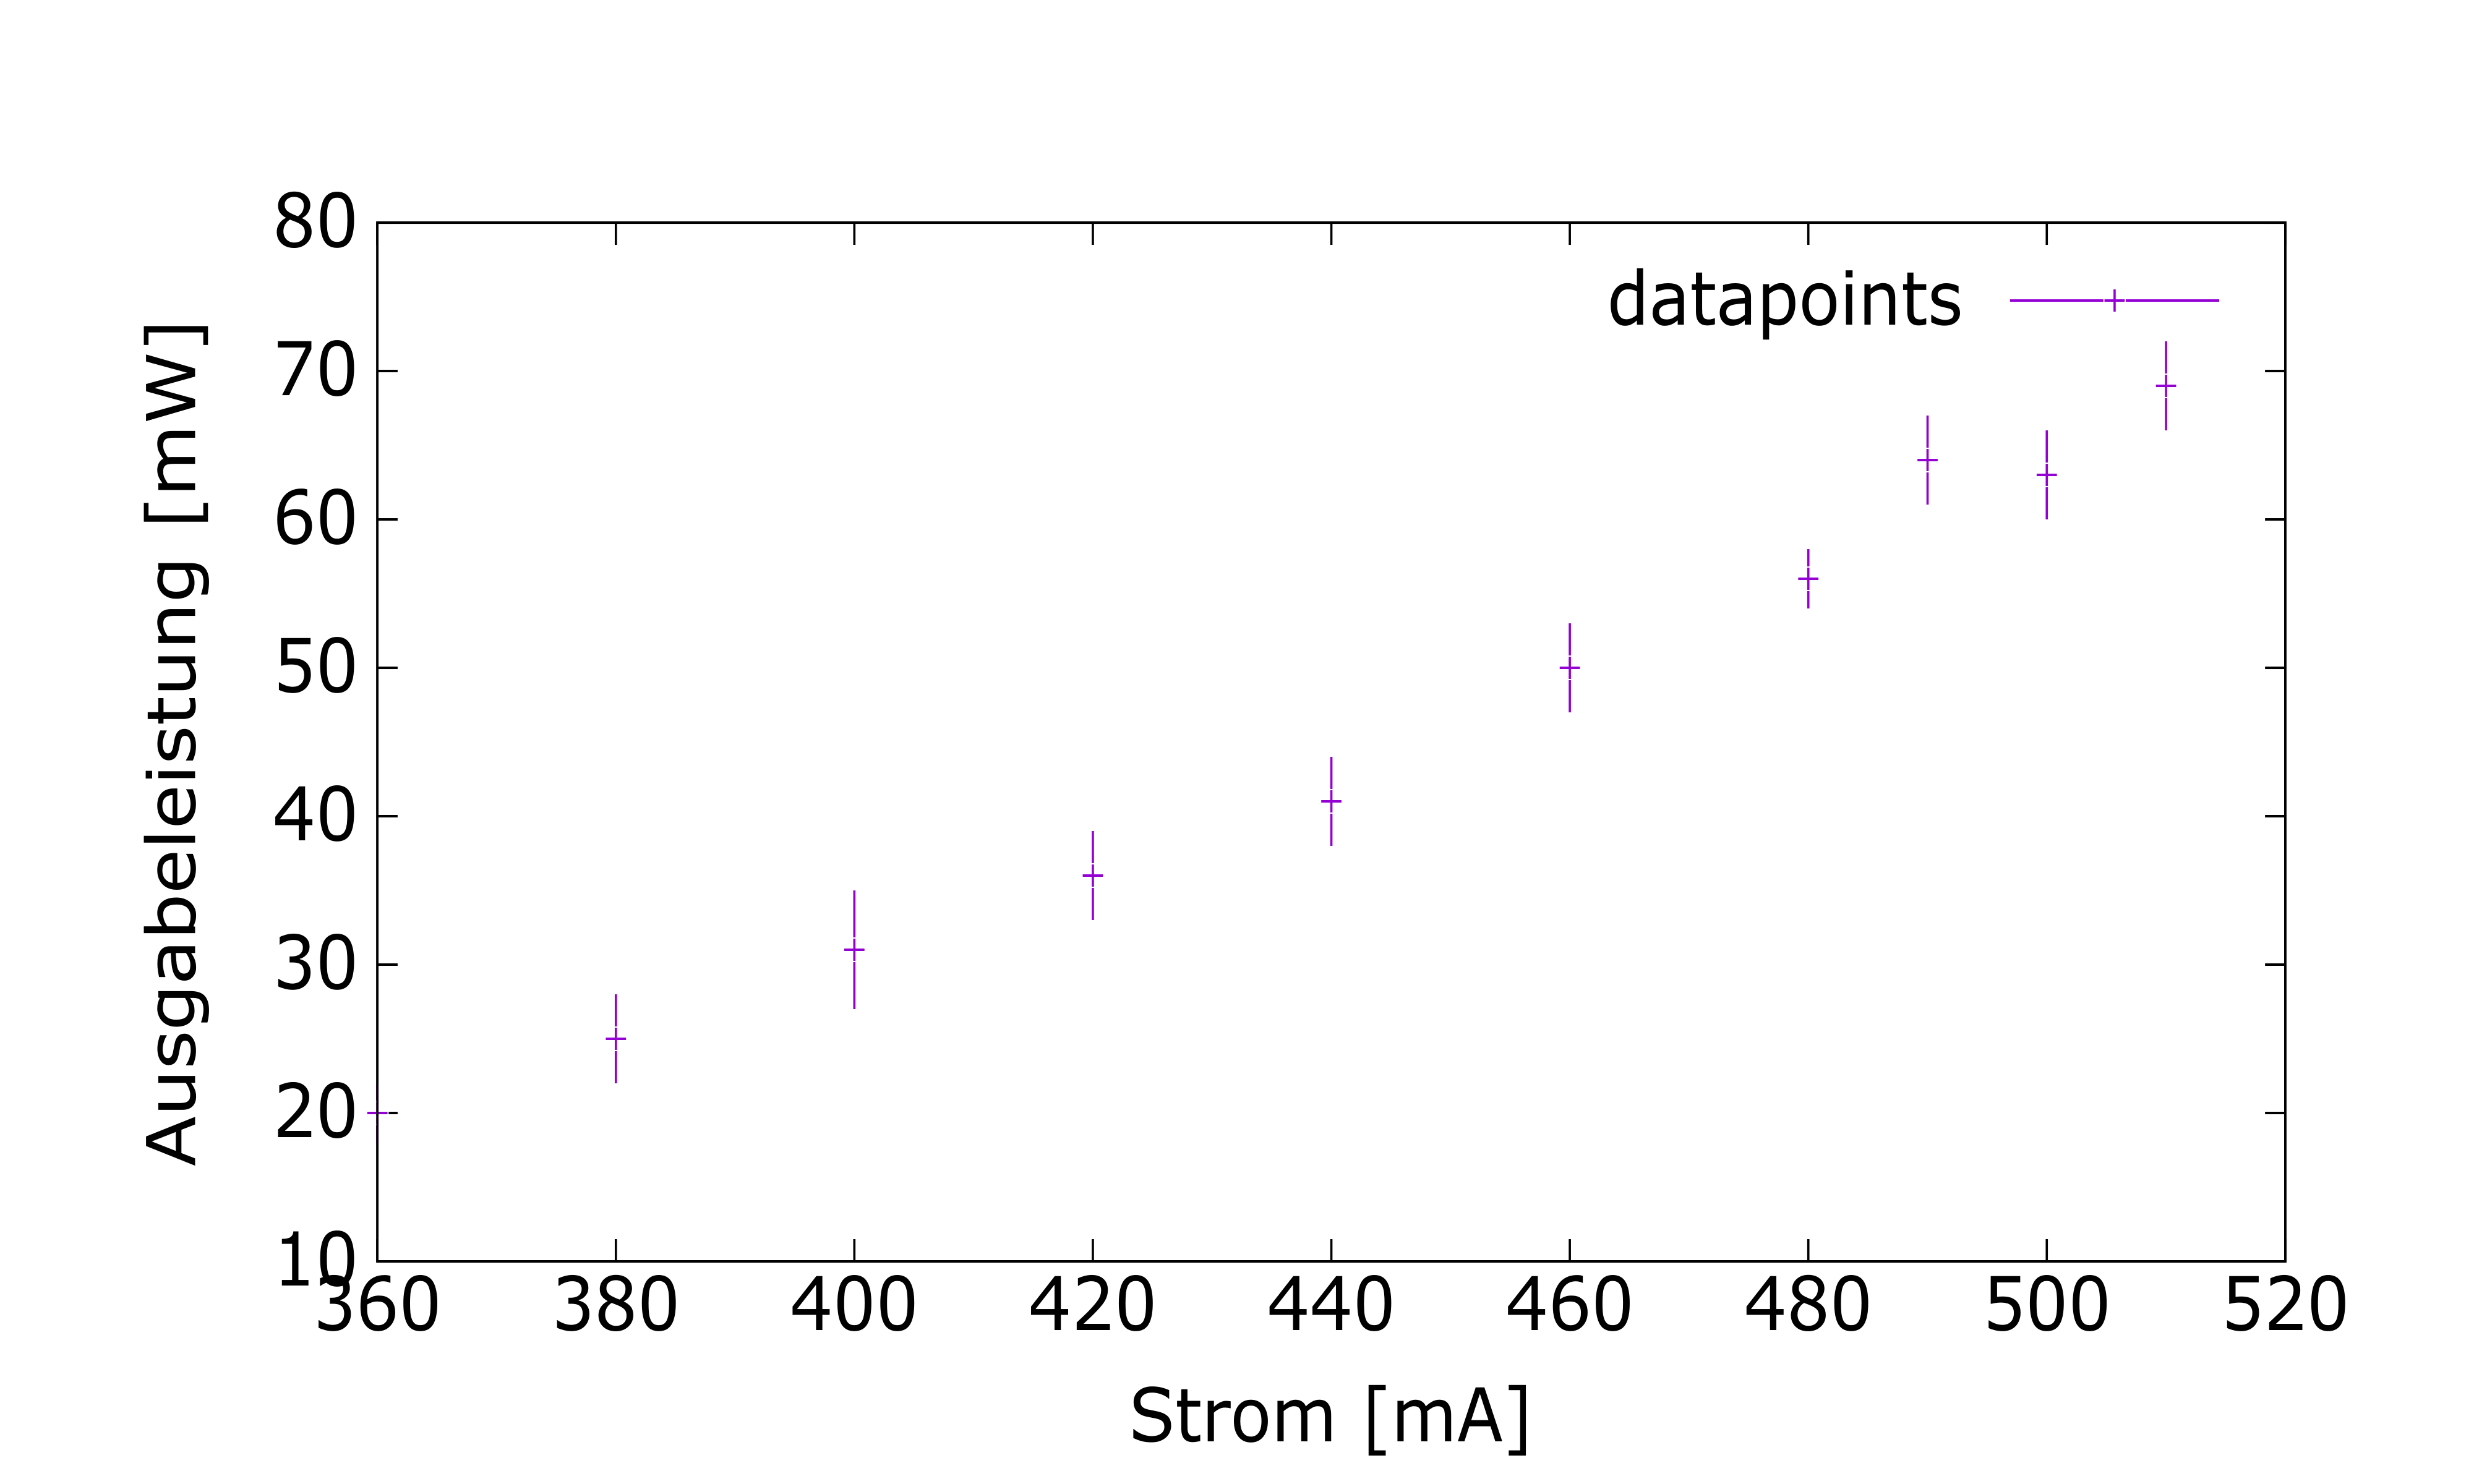
\includegraphics[width=\textwidth]{../../Bilddateien/1-2/Rasterung_30deg.png}
    %%         \caption{Rasterung um $30\si{\celsius}$.}
    %%         \label{fig:1-2:Rasterung30deg}
    %%     \end{subfigure}
    %%     \caption{Die Transmissionsleistung zu fester Temperatur $T\in\mcT$ als Funktion der Anregungsleistung $P_{\textit{an}}$.}
    %% \end{figure}
    Die technische Ausführung dieses Versuchsteils mit dem Ziel der Untersuchung einer Beziehung zwischen gewählter Diodenlasertemperatur und des Diodenlaserstroms zum Erhalt einer konstanten, durch die physikalische Eigenschaften des Nd:YAG Kristall gegebenen Wellenlänge $\lambda = 808\si{\nm}$ wurde von uns im Verlaufe des Teils von der Rasterung über den Strom $I$ bei konstanter Temperatur $T$ zur Rasterung über die Temperatur $T$ bei konstantem Strom $I$ geändert, da auf diese Weise die Transmissionsleistungsminima in $P_{t,i}$ besser erkennbar waren.

    Somit Minimieren wir die Abbildung $T\mapsto P_{t,i}(T)$ mit festen Stromwerten $I_i\in\{50\si{\mA},150\si{\mA},250\si{\mA},350\si{\mA},450\si{\mA},550\si{\mA}\}=:\mcI$ und $P_{t,i}:=P_t(I_i)$ als Abzählung $I:[6]\to\mcI$, was eine Charakterisierung der Kennlinie ermöglicht. Für verschiedene $i\in[6]$ erhalten wir so bestimmte Parameter $T_{0,i}:=T_0(I_i)$, welche in $P_{t,i}$ ein Minimum erzeugen. Zur Darstellung zeichnen wir dieses $T_0(i)$ als Funktion des Eingabestroms $I_i$ in Form der gesuchten Kennlinie auf. Das Ergebnis der Messreihe ist in Abbildung \ref{fig:1-2:RasterungEvalMinChgI} gegeben. Eine Kurvenanpassung mittels linearen Zusammenhangs $f_{a,b}(x) := a\cdot x + b$ liefert uns die Parametertabelle \ref{tab:1-2:RasterungEvalMinChgI} mit Parametern $a,b$ und ihren zugehörig berechneten asymptotischen Standardunsicherheiten $u(a),u(b)$.

    \begin{figure}[H]
        \centering
        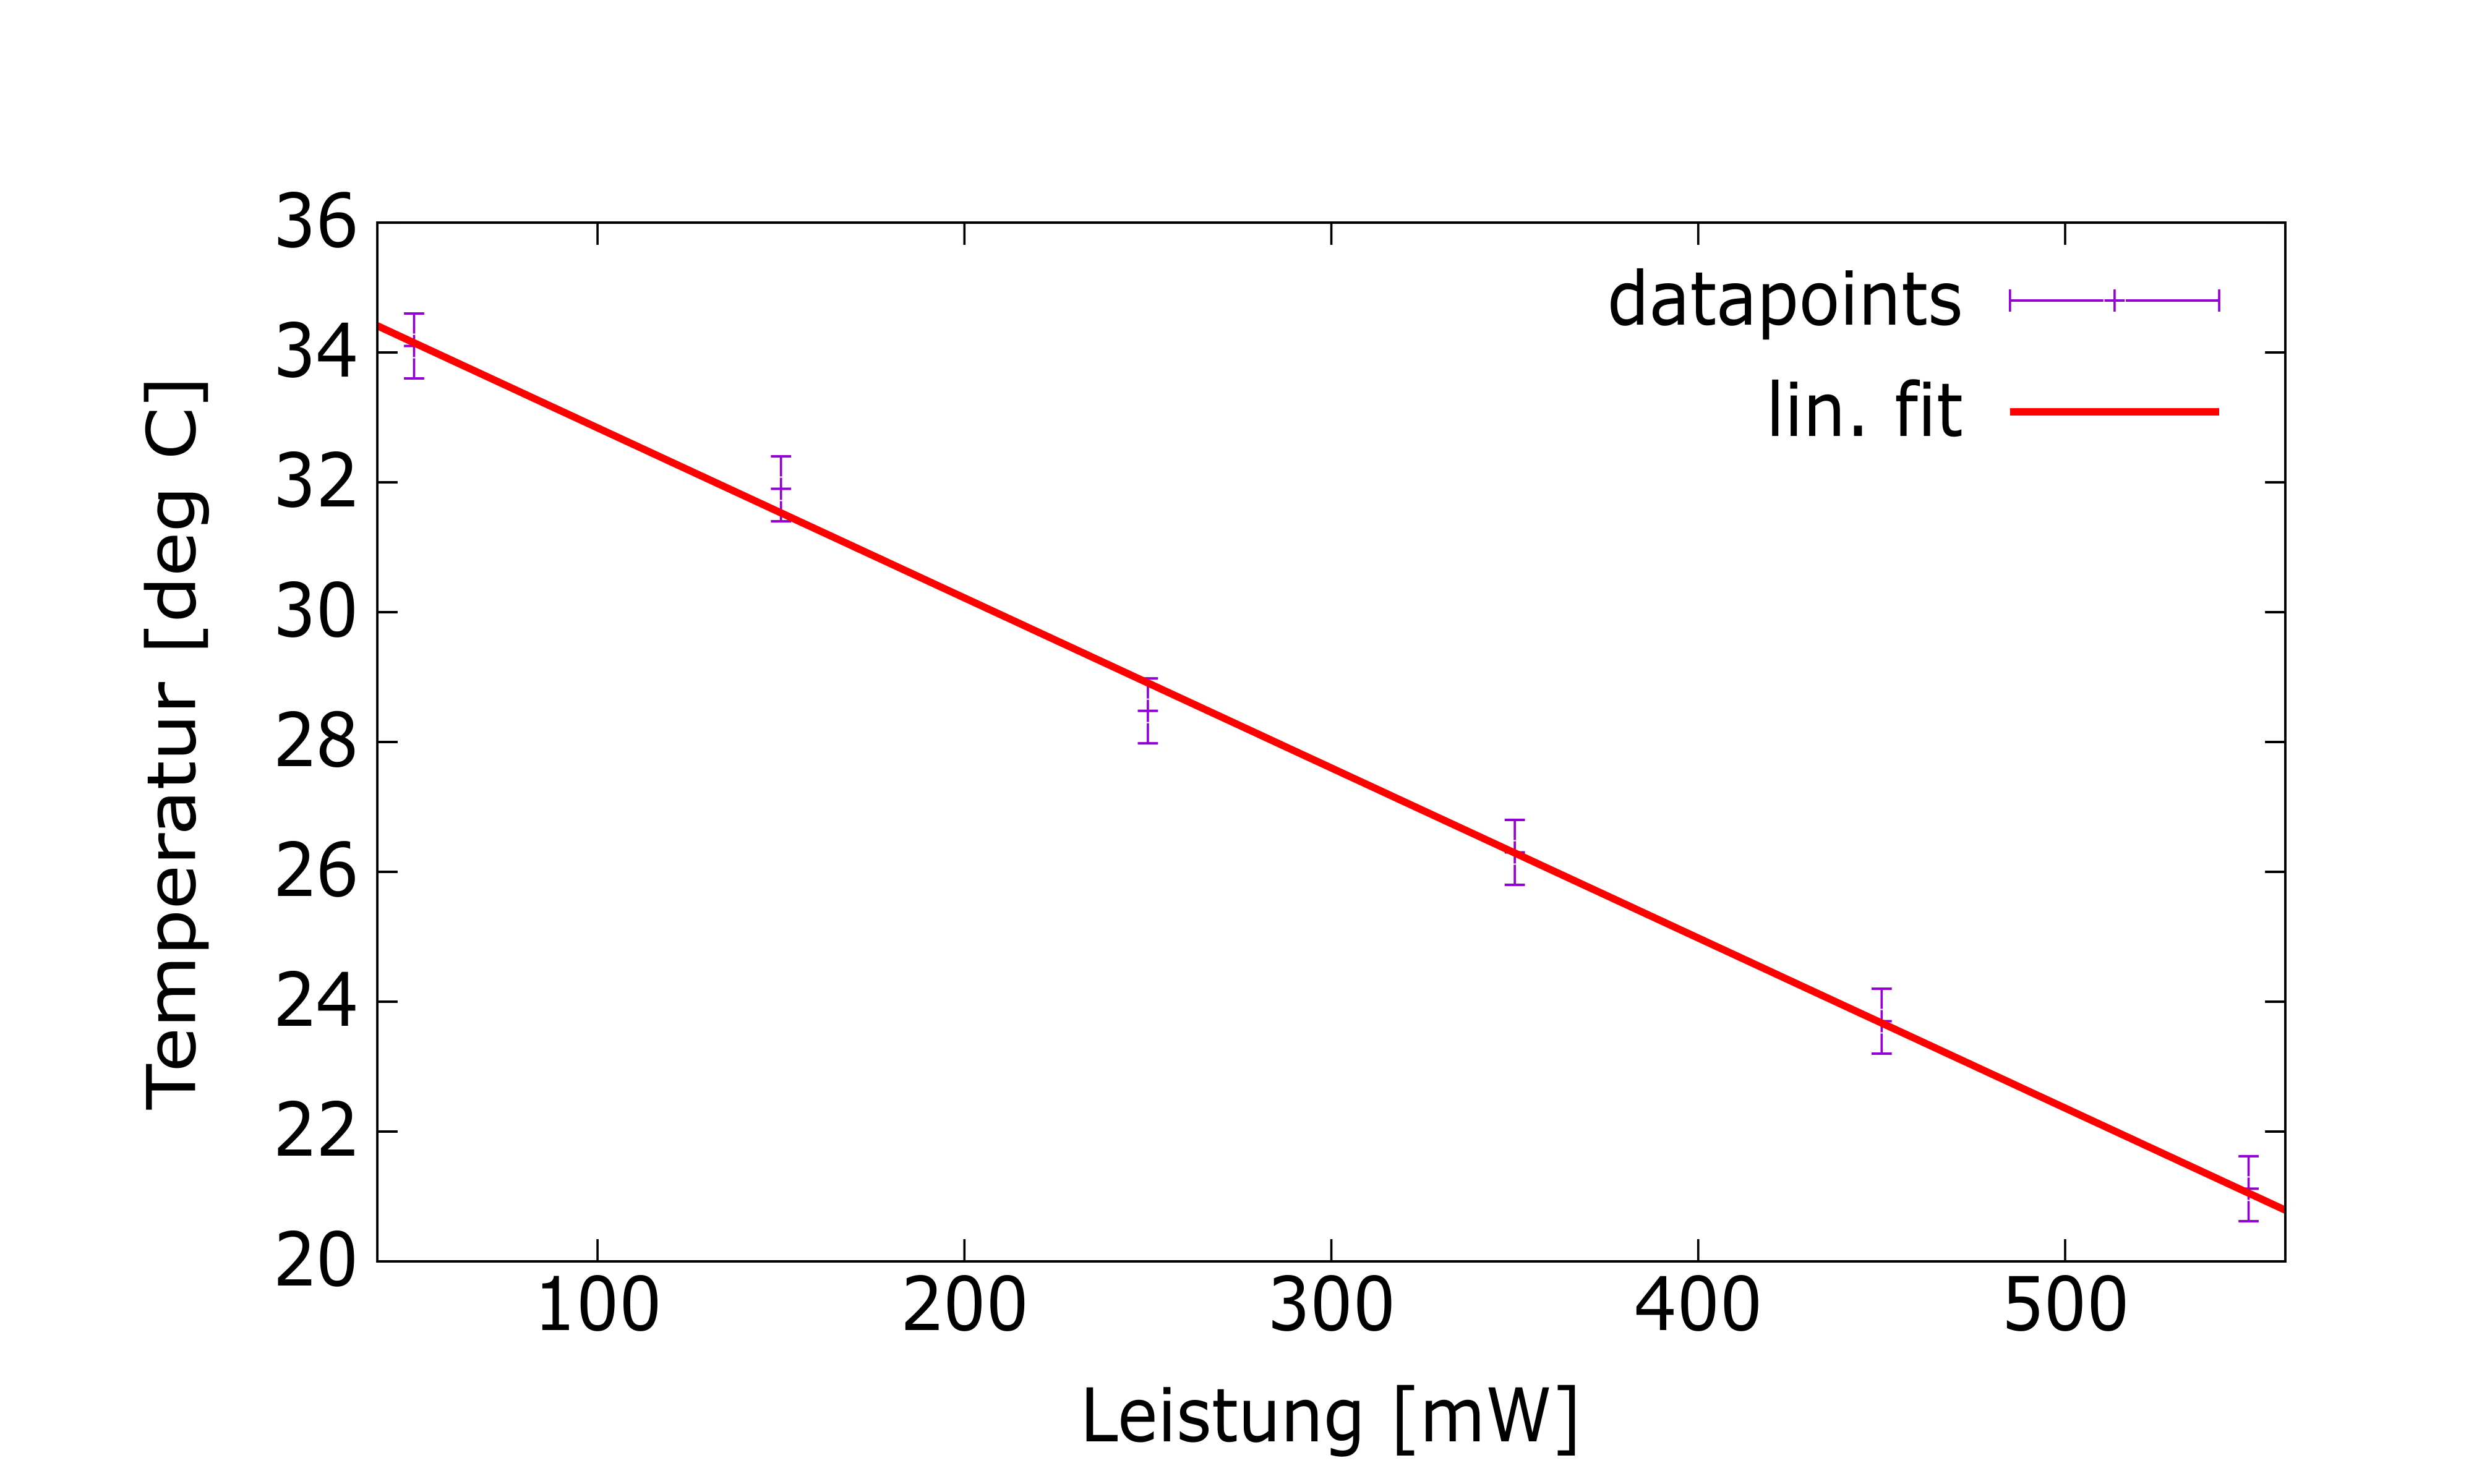
\includegraphics[width=11cm]{../../Bilddateien/1-2/Rasterung_EvalMin_chgI.png}
        \caption{Die optimierende Temperatur $T_0$ als Funktion des Anregungsstroms $I_{\textit{an}}$.}
        \label{fig:1-2:RasterungEvalMinChgI}
    \end{figure}

    \begin{table}[H]
        \centering
        \begin{tabular}{c|cc|cc}
            \hline
            & $a$ in $\si{\celsius\per\W}$ & $u(a)$ in $\si{\celsius\per\W}$ & $b$ in $\si{\celsius}$ & $u(b)$ in $\si{\celsius}$ \\
            \hline\hline
            $f_{a,b}$ & $-26.1943$ & $0.6868$ & $35.4583$ & $0.2371$ \\
            \hline
        \end{tabular}
    \end{table}
    Als Charakterisierung des Fits bezüglich der gegebenen Messdaten wählen wir die Methode der \emph{residual sum of squares} (RSS), welche uns den Wert $RSS(f_{a,b}) = 0.330194$ liefert. 
\end{document}